% ============================================================
%  FPGA-Accelerated Network IDS — IDS Chapter
%  Matching style: report class, Computer Modern, justified
%  Authors: Youcef Slimani & Salah Eddine Laifa
%  M'Hamed Bougara University of Boumerdes — May 2026
% ============================================================

\documentclass[12pt, a4paper]{report}

% --- Packages ---
\usepackage[T1]{fontenc}
\usepackage[utf8]{inputenc}
\usepackage{lmodern}
\usepackage[a4paper, top=2.5cm, bottom=2.5cm, left=3cm, right=2.5cm]{geometry}
\usepackage{graphicx}
\usepackage{booktabs}
\usepackage{array}
\usepackage{tabularx}
\usepackage{longtable}
\usepackage{listings}
\usepackage{xcolor}
\usepackage{amsmath}
\usepackage{fancyhdr}
\usepackage{titlesec}
\usepackage{hyperref}
\usepackage{caption}
\usepackage{float}
\usepackage{setspace}
\usepackage{emptypage}
\usepackage{tocloft}

% --- Hyperref setup ---
\hypersetup{
    colorlinks=true,
    linkcolor=black,
    citecolor=black,
    urlcolor=blue,
    pdfauthor={Youcef Slimani, Salah Eddine Laifa},
    pdftitle={FPGA-Accelerated Network IDS with RISC-V Co-Processor Integration},
}

% --- Chapter title style (matching reference document) ---
\titleformat{\chapter}[display]
  {\normalfont\huge\bfseries}
  {\chaptertitlename\ \thechapter}
  {20pt}
  {\Huge}
\titlespacing*{\chapter}{0pt}{50pt}{40pt}

% --- Section/subsection style ---
\titleformat{\section}{\normalfont\Large\bfseries}{\thesection}{1em}{}
\titleformat{\subsection}{\normalfont\large\bfseries}{\thesubsection}{1em}{}
\titleformat{\subsubsection}{\normalfont\normalsize\bfseries}{\thesubsubsection}{1em}{}

% --- Header/footer ---
\pagestyle{fancy}
\fancyhf{}
\fancyhead[R]{\itshape\leftmark}
\fancyfoot[C]{\thepage}
\renewcommand{\headrulewidth}{0.4pt}
\fancypagestyle{plain}{
  \fancyhf{}
  \fancyfoot[C]{\thepage}
  \renewcommand{\headrulewidth}{0pt}
}

% --- VHDL listing style ---
\lstdefinelanguage{VHDL}{
  morekeywords={library,use,entity,port,architecture,signal,process,
    begin,end,if,then,else,elsif,case,when,others,in,out,inout,
    std_logic,std_logic_vector,unsigned,integer,is,of,type,
    rising_edge,to_integer,to_unsigned,downto,variable,null,
    generic,map,not,and,or,xor,nor,nand,xnor,all},
  sensitive=false,
  morecomment=[l]{--},
  morestring=[b]",
}

\lstset{
  language=VHDL,
  basicstyle=\ttfamily\footnotesize,
  keywordstyle=\bfseries,
  commentstyle=\itshape\color{gray},
  stringstyle=\color{darkgray},
  numbers=left,
  numberstyle=\tiny\color{gray},
  stepnumber=1,
  frame=single,
  breaklines=true,
  tabsize=4,
  captionpos=b,
}

% --- Table of contents depth ---
\setcounter{tocdepth}{2}
\setcounter{secnumdepth}{3}

% ============================================================
\begin{document}

% ============================================================
%  TITLE PAGE
% ============================================================
\begin{titlepage}
\centering

\vspace*{1.5cm}
{\Huge\bfseries FPGA-Accelerated Network IDS with\\[0.4em] RISC-V Co-Processor Integration\par}

\vspace{2.5cm}

\includegraphics[width=5cm]{logo.pdf}

\vspace{2.5cm}
{\large Youcef Slimani\\Salah Eddine Laifa\par}

\vspace{1cm}
{\normalsize
Institute of Electrical and Electronic Engineering\\
Fundamental Teaching Department\\
M'Hamed Bougara University of Boumerdes\par}

\vfill
{\normalsize Submitted in partial satisfaction of the requirements for the\\
Degree of Bachelor\\
in Electrical and Electronic Engineering\par}

\vspace{1cm}
{\normalsize\itshape Supervisor\hspace{1em} Dr.~Touzzout Walid\par}

\vspace{1cm}
{\normalsize May 2026\par}
\end{titlepage}

% ============================================================
%  FRONT MATTER
% ============================================================
\pagenumbering{roman}

% --- Dedications ---
\chapter*{Dedications}
\addcontentsline{toc}{chapter}{Dedications}

This thesis is dedicated to our families for their endless support and encouragement throughout our studies.

We further dedicate this work to all our colleagues and teachers who contributed to our academic journey.

\clearpage

% --- Acknowledgements ---
\chapter*{Acknowledgements}
\addcontentsline{toc}{chapter}{Acknowledgements}

We would like to express our deepest gratitude to our supervisor, Dr.~Touzzout Walid, for his invaluable guidance, patience, and constant encouragement throughout this project.

We would also like to thank the IGEE (ex.~INELEC) department for providing the necessary facilities and resources.

\clearpage

% --- Abstract ---
\chapter*{Abstract}
\addcontentsline{toc}{chapter}{Abstract}

This thesis presents a hardware-based Network Intrusion Detection System (IDS) implemented on the programmable logic of a Zynq-7020 FPGA, integrated with a RISC-V co-processor developed by a parallel project. The IDS inspects every incoming Ethernet frame at wire speed, extracting header fields from the Ethernet, IPv4, TCP, and UDP layers and evaluating them against a set of twenty detection rules. All rule evaluations complete in a single clock cycle, giving the system a deterministic, constant-latency response to every packet regardless of traffic volume.

The hardware design is described in VHDL and verified through behavioural simulation in Vivado. The integration architecture couples the IDS pipeline to the BigDCore RISC-V processor through a memory-mapped shared register bank: the IDS continuously writes threat data and alert flags, while the RISC-V reads these values to decide alert severity, update detection thresholds at runtime, and transmit formatted alerts over UART.

\textbf{Keywords:} FPGA, VHDL, Intrusion Detection System, Zynq-7020, RISC-V, network security, hardware acceleration, Vivado.

\clearpage

% --- Table of Contents ---
\tableofcontents
\clearpage

% --- List of Figures ---
\listoffigures
\clearpage

% --- List of Tables ---
\listoftables
\clearpage

% ============================================================
%  MAIN MATTER
% ============================================================
\pagenumbering{arabic}

% ============================================================
\chapter{Introduction}
% ============================================================

Network traffic volumes and attack sophistication have grown to a point where software intrusion detection systems face fundamental throughput limitations. A software IDS running on a general-purpose CPU must copy packet data through the OS network stack, schedule the inspection process, and share the CPU with other tasks---all of which introduce variable latency and reduce the fraction of packets that can actually be inspected at high line rates.

Reconfigurable hardware offers a different trade-off: inspection logic is implemented directly as digital circuits in an FPGA, so packets are examined as bytes arrive, with no operating system, no scheduling overhead, and no data copies. The cost is development complexity; the benefit is deterministic, wire-speed inspection.

This project builds a hardware IDS in VHDL, targeting the MicroPhase Z7-Lite development board (Zynq-7020, XC7Z020-1CLG400C), and integrates it with a RISC-V processor built independently by a collaborator. The Zynq device is a natural fit: its ARM Cortex-A9 Processing System (PS) receives Ethernet packets through the on-chip GigE MAC and can forward raw frame data to the Programmable Logic (PL) fabric via AXI-Stream DMA, where the IDS pipeline runs. The RISC-V processor also resides in the PL fabric and communicates with the IDS through a shared memory-mapped register bank.

The IDS is developed and validated entirely through behavioural simulation before any hardware integration, allowing each layer of the protocol stack to be verified independently with injected test packets.

\section{Project Scope}

The IDS component of this project is responsible for:
\begin{itemize}
    \item Receiving a raw byte stream representing Ethernet frames.
    \item Parsing Ethernet, IPv4, TCP, and UDP headers.
    \item Evaluating twenty detection rules spanning four protocol layers.
    \item Accumulating a weighted threat score and classifying traffic severity.
    \item Exposing all status data and configurable rule parameters to the RISC-V co-processor through a shared register bank.
\end{itemize}

Hardware integration (block design, AXI-Stream DMA, PS bare-metal driver) constitutes the deployment path and is described in Chapter~\ref{ch:integration}.

\section{Document Structure}

Chapter~\ref{ch:architecture} describes the IDS pipeline architecture and the design of each VHDL module. Chapter~\ref{ch:rules} lists all twenty detection rules and the reasoning behind each one. Chapter~\ref{ch:simulation} presents the simulation methodology and results. Chapter~\ref{ch:integration} covers the integration architecture with the RISC-V co-processor and the hardware deployment plan. Chapter~\ref{ch:conclusion} concludes with a summary of achievements and directions for future work.

% ============================================================
\chapter{IDS Pipeline Architecture}
\label{ch:architecture}
% ============================================================

\section{Design Philosophy}

The IDS is structured as a linear pipeline of independent modules, each consuming the same byte stream that flows from a physical interface receiver. Parsers at different protocol layers operate simultaneously on the same data; rule checkers fire one clock cycle after their corresponding parser completes. This means the system does not buffer a full packet before beginning inspection---field extraction and rule evaluation are interleaved with frame reception.

The choice of a byte-stream interface as the internal contract between modules makes each module independently testable and allows the physical reception mechanism to be swapped (from RMII simulation to AXI-Stream DMA for hardware) without modifying any parser or checker.

\section{Top-Level Structure}

The pipeline is wired together in a single top-level entity, \texttt{ids\_top.vhd}. It instantiates all sub-modules and connects them through internal signals. The byte stream---\texttt{rx\_byte}, \texttt{rx\_valid}, \texttt{rx\_sof}, \texttt{rx\_eof}---is broadcast to every parser simultaneously.

% --- FIGURE PLACEHOLDER ---
% Replace with the IDS pipeline diagram (Image 1 from your PNGs)
%
 \begin{figure}[H]
     \centering
     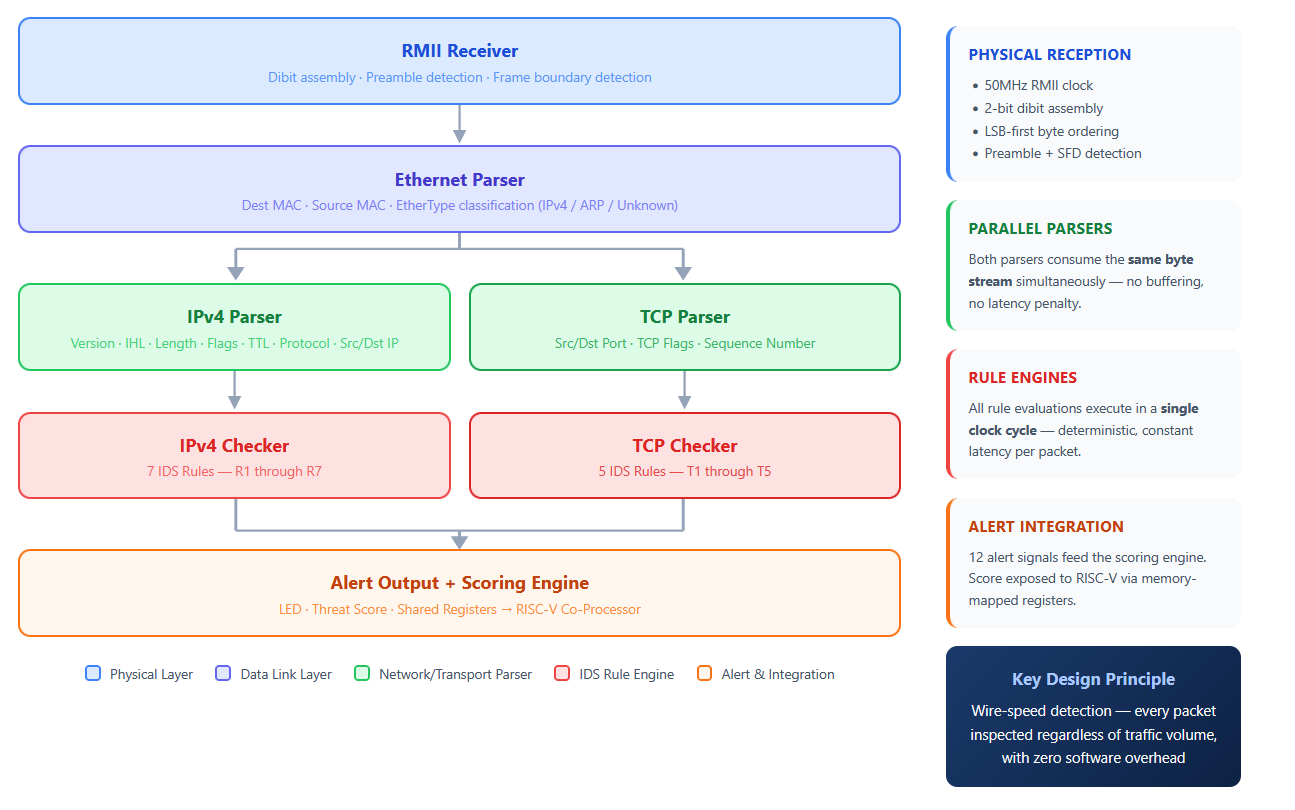
\includegraphics[width=0.95\textwidth]{ids_pipeline_diagram.png}
     \caption{IDS pipeline architecture showing parallel parsers and rule engines.}
     \label{fig:pipeline}
 \end{figure}

\noindent The four-signal byte-stream interface carries the following semantics:
\begin{itemize}
    \item \texttt{rx\_sof} pulses for one clock cycle at the start of a new frame.
    \item \texttt{rx\_byte} / \texttt{rx\_valid} delivers one byte per clock when valid.
    \item \texttt{rx\_eof} pulses for one clock cycle at the end of the frame.
\end{itemize}

This interface is the internal standard across all modules.

\section{RMII Receiver (\texttt{rmii\_rx.vhd})}

In simulation, Ethernet frames are injected using RMII signalling: two data bits (a \emph{dibit}) are presented every clock cycle at 50\,MHz, LSB-first. The RMII receiver is a three-state FSM (IDLE, PREAMBLE, DATA) that assembles four consecutive dibits into one byte using a right-shift register:

\begin{lstlisting}[caption={Dibit assembly in \texttt{rmii\_rx.vhd}}, label=lst:rmii]
shift_reg <= rmii_rxd & shift_reg(7 downto 2);
if dibit_cnt = "11" then
    rx_byte  <= rmii_rxd & shift_reg(7 downto 2);
    rx_valid <= '1';
end if;
\end{lstlisting}

The preamble state counts at least eight \texttt{01} dibits before accepting the Start Frame Delimiter (\texttt{11}). On hardware, this module is replaced by an AXI-Stream receiver that accepts bytes directly from the PS DMA engine; the rest of the pipeline is unchanged.

\section{Ethernet Parser (\texttt{eth\_parser.vhd})}

The Ethernet parser extracts the destination MAC, source MAC, and EtherType from the first 14 bytes of each frame. It uses a sequential FSM with states for each header field group (DST\_MAC, SRC\_MAC, ETHERTYPE, PAYLOAD, DONE). On the DONE state, it asserts \texttt{frame\_done} and one of \texttt{is\_ipv4}, \texttt{is\_arp}, or \texttt{is\_unknown} based on the EtherType value (0x0800, 0x0806, or other).

A key design decision is that all output signals default to \texttt{'0'} at the top of the clocked process and are only overridden in the DONE state. This prevents latches and ensures outputs are valid for exactly one clock cycle.

\section{Frame Counter (\texttt{frame\_counter.vhd})}

The frame counter accumulates per-second frame statistics (total, IPv4, ARP, unknown) using a hardware divider: a counter incremented every clock cycle triggers a \texttt{one\_sec\_tick} when it reaches \texttt{CLK\_FREQ\_HZ - 1}. On that tick, the running accumulators are latched to output registers and reset. This value is passed as a generic so the same code simulates at \texttt{CLK\_FREQ\_HZ = 1000} (1\,kHz) and synthesizes at \texttt{CLK\_FREQ\_HZ = 50\,000\,000} (50\,MHz), making testbenches fast without any code changes.

\section{IPv4 Parser (\texttt{ipv4\_parser.vhd})}

The IPv4 parser skips the 14-byte Ethernet header (counted in the ETH\_HEADER state) and then extracts the following fields from the IP header:

\begin{table}[H]
\centering
\caption{IPv4 header fields extracted by \texttt{ipv4\_parser.vhd}}
\label{tab:ipv4fields}
\begin{tabular}{lll}
\toprule
\textbf{Field} & \textbf{Byte offset} & \textbf{Width} \\
\midrule
Version / IHL   & 0      & 4 + 4 bits \\
Total Length    & 2--3   & 16 bits    \\
Flags / Fragment Offset & 6--7 & 3 + 13 bits \\
TTL             & 8      & 8 bits     \\
Protocol        & 9      & 8 bits     \\
Source IP       & 12--15 & 32 bits    \\
Destination IP  & 16--19 & 32 bits    \\
\bottomrule
\end{tabular}
\end{table}

The IHL field determines where the IP header ends (IHL\,$\times$\,4 bytes). The parser computes this boundary dynamically and transitions to WAIT\_EOF once all header bytes have been consumed, asserting \texttt{parse\_done} and \texttt{parse\_valid} (the latter only when \texttt{ip\_version = 4}) after the frame ends.

\section{IPv4 Checker (\texttt{ipv4\_checker.vhd})}

The IPv4 checker receives the parsed fields when \texttt{parse\_done} is asserted and evaluates all rules combinatorially inside a clocked process in a single clock cycle. A local variable \texttt{any\_alert} is OR'd across all rule conditions and drives the \texttt{alert\_any} output. Individual alert signals (\texttt{alert\_bad\_version}, \texttt{alert\_fragment}, etc.) are also driven, allowing the scoring engine to weight them differently.

\section{TCP Parser (\texttt{tcp\_parser.vhd})}

The TCP parser shares the same byte stream as the IPv4 parser. Because the TCP header begins at a byte offset that depends on the IP IHL field, the parser captures \texttt{ip\_ihl} and \texttt{ip\_protocol} from the IPv4 parser's output signals before the frame starts. It then skips to byte \texttt{14 + IHL\,$\times$\,4} (Ethernet header + IP header) before beginning TCP field extraction.

Fields extracted: source port, destination port, sequence number, and the flags byte. The flags byte at offset 13 of the TCP header encodes FIN, SYN, RST, PSH, ACK, and URG in bits 0--5.

\section{TCP Checker (\texttt{tcp\_checker.vhd})}

The TCP checker uses VHDL \texttt{alias} declarations to give readable names to individual flag bits:

\begin{lstlisting}[caption={Flag aliases in \texttt{tcp\_checker.vhd}}, label=lst:aliases]
alias flag_fin : std_logic is tcp_flags(0);
alias flag_syn : std_logic is tcp_flags(1);
alias flag_rst : std_logic is tcp_flags(2);
\end{lstlisting}

Rules are expressed directly as Boolean conditions on these aliases, making the intent clear without bit-masking arithmetic.

\section{UDP Parser (\texttt{udp\_parser.vhd})}

The UDP header is 8 bytes long: source port (2), destination port (2), length (2), and checksum (2). The parser reuses the same skip-to-transport-layer logic as the TCP parser, activated only when \texttt{ip\_protocol = 0x11}. The \texttt{parse\_valid} output is asserted only for UDP packets.

\section{UDP Checker (\texttt{udp\_checker.vhd})}

The UDP checker evaluates nine rules on the extracted UDP fields and a configurable set of forbidden port values, shared with the TCP checker through the rule register bank.

% ============================================================
\chapter{Detection Rules}
\label{ch:rules}
% ============================================================

\section{Overview}

The IDS evaluates twenty detection rules across four protocol layers. Rules are grouped by the checker module that evaluates them. Each rule fires for exactly one clock cycle when its condition is met; the alert is latched and its weight added to the threat score.

\section{IPv4 Rules (R1--R12)}

\subsection{Rules R1--R7: Core Validity Checks}

These seven rules detect structurally malformed or trivially suspicious IPv4 packets.

\begin{table}[H]
\centering
\caption{IPv4 detection rules R1--R7}
\label{tab:r1r7}
\begin{tabular}{lll}
\toprule
\textbf{Rule} & \textbf{Condition} & \textbf{Attack / Anomaly} \\
\midrule
R1 & \texttt{ip\_version} $\neq$ 4          & Non-IPv4 / malformed packet \\
R2 & \texttt{ip\_ihl} $<$ 5                  & Invalid header length       \\
R3 & \texttt{ip\_length} $<$ 20              & Impossible packet size      \\
R4 & \texttt{ip\_ttl} $\leq$ 1              & Suspicious TTL / traceroute \\
R5 & \texttt{ip\_frag\_off} $>$ 0           & Fragmentation attack        \\
R6 & \texttt{ip\_src} = \texttt{0.0.0.0}   & Spoofed source address      \\
R7 & \texttt{ip\_src} = \texttt{ip\_dst}   & Land attack                 \\
\bottomrule
\end{tabular}
\end{table}

\subsection{Rules R8--R12: Bogon and Header Abuse}

These five rules detect packets whose source addresses belong to reserved or unroutable address blocks, or whose header fields abuse optional mechanisms.

\begin{table}[H]
\centering
\caption{IPv4 detection rules R8--R12}
\label{tab:r8r12}
\begin{tabular}{lll}
\toprule
\textbf{Rule} & \textbf{Condition} & \textbf{Attack / Anomaly} \\
\midrule
R8  & \texttt{ip\_src[31:24]} = \texttt{0x7F}          & Loopback source (127.x.x.x)        \\
R9  & \texttt{ip\_src[31:16]} = \texttt{0xA9FE}        & Link-local source (169.254.x.x)    \\
R10 & \texttt{ip\_src[31:28]} = \texttt{0xE}           & Multicast source (224--239.x.x.x) \\
R11 & \texttt{ip\_ihl} $>$ 5                           & IP options present                  \\
R12 & \texttt{ip\_flags[2]} = \texttt{'1'}             & Reserved IPv4 flag bit set          \\
\bottomrule
\end{tabular}
\end{table}

Rules R8--R10 share a single enable bit (\texttt{bogon\_check\_en}) in the rule register bank so the RISC-V can disable them all at once on a network segment where such addresses may legitimately appear.

\section{TCP Rules (T1--T5)}

\begin{table}[H]
\centering
\caption{TCP detection rules T1--T5}
\label{tab:t1t5}
\begin{tabular}{lll}
\toprule
\textbf{Rule} & \textbf{Condition} & \textbf{Attack / Anomaly} \\
\midrule
T1 & SYN = 1 and FIN = 1                    & Illegal flag combination    \\
T2 & SYN = 1 and RST = 1                    & Illegal flag combination    \\
T3 & All flags = \texttt{0x00}              & NULL scan (port probe)      \\
T4 & All flags = \texttt{0xFF}              & XMAS scan (port probe)      \\
T5 & \texttt{dst\_port} $\in$ forbidden set & Access to forbidden service \\
\bottomrule
\end{tabular}
\end{table}

The forbidden port set (rule T5) is stored in configurable registers and defaults to Telnet (23), FTP (21), and TFTP (69). The RISC-V processor can update these values without reprogramming the FPGA.

\section{UDP Rules (U1--U9)}

\begin{table}[H]
\centering
\caption{UDP detection rules U1--U9}
\label{tab:u1u9}
\begin{tabular}{lp{6cm}p{6cm}}
\toprule
\textbf{Rule} & \textbf{Condition} & \textbf{Attack / Anomaly} \\
\midrule
U1 & \texttt{udp\_dst\_port} $\in$ forbidden set & Access to forbidden UDP service \\
U2 & \texttt{udp\_length} $<$ 8 & Invalid UDP length field \\
U3 & \texttt{udp\_length} $=$ 0 & Completely malformed UDP packet \\
U4 & \texttt{udp\_src\_port} $\in$ \{53, 123, 11211, 19\} & Amplification attack response (DNS/NTP/Memcached/CHARGEN) \\
U5 & \texttt{ip\_src} $=$ \texttt{ip\_dst} $\wedge$ \texttt{udp\_src\_port} $=$ \texttt{udp\_dst\_port} & UDP land attack \\
U6 & \texttt{udp\_length} $>$ 1472 & Oversized datagram (exceeds Ethernet MTU) \\
U7 & \texttt{udp\_src\_port} $=$ 0 $\vee$ \texttt{udp\_dst\_port} $=$ 0 & Reserved port zero used \\
U8 & \texttt{udp\_dst\_port} $=$ 1900 & SSDP/UPnP abuse \\
U9 & \texttt{udp\_dst\_port} $=$ 11211 & Memcached amplification request \\
\bottomrule
\end{tabular}
\end{table}
\newpage
\section{Alert Weighting}

Each alert type is assigned a weight, and the scoring engine accumulates weights additively. The RISC-V classifies traffic into three severity tiers based on the accumulated score.
\begin{table}[H]
\centering
\caption{Alert weights used by the scoring engine}
\label{tab:weights}
\begin{tabular}{llr}
\toprule
\textbf{Alert} & \textbf{Rule} & \textbf{Weight} \\
\midrule
Bad version          & R1       & 5  \\
Bad IHL              & R2       & 5  \\
Bad length           & R3       & 10 \\
Low TTL              & R4       & 5  \\
Fragmentation        & R5       & 15 \\
Spoofed source       & R6       & 20 \\
Land attack          & R7       & 25 \\
Bogon source         & R8--R10  & 15 \\
IP options           & R11      & 10 \\
Reserved flag        & R12      & 10 \\
SYN+FIN              & T1       & 25 \\
SYN+RST              & T2       & 20 \\
NULL scan            & T3       & 20 \\
XMAS scan            & T4       & 20 \\
Forbidden TCP port   & T5       & 15 \\
Forbidden UDP port   & U1       & 15 \\
Malformed UDP length & U2, U3   & 10 \\
Amplification resp.  & U4       & 20 \\
UDP land attack      & U5       & 25 \\
Oversized UDP        & U6       & 10 \\
Port zero            & U7       & 10 \\
SSDP/UPnP abuse      & U8       & 15 \\
Memcached amplif.    & U9       & 20 \\
\bottomrule
\end{tabular}
\end{table}

The score decays by a configurable rate every second when no new alerts fire, preventing a historical event from permanently elevating the severity level.

% ============================================================
\chapter{Simulation and Verification}
\label{ch:simulation}
% ============================================================

\section{Methodology}

Each checker module is verified independently before the full-pipeline testbench is run. The testbench for a given checker instantiates only the relevant parser--checker pair, injects synthetic byte streams that exercise boundary conditions, and verifies alert signals in the simulation waveform. This makes debugging straightforward: a failing assertion on \texttt{alert\_syn\_fin} in \texttt{tcp\_checker\_tb} is isolated from anything happening in the Ethernet or IP layers.

The full-pipeline testbench (\texttt{ids\_top\_tb.vhd}) then exercises the entire chain from RMII dibit injection to alert latch, confirming that parser outputs are correctly connected as checker inputs and that the alert latch persists across frames.

A critical testbench optimisation is the use of a reduced clock frequency generic:

\begin{lstlisting}[caption={Generic override in the testbench}, label=lst:generic]
u_dut : entity work.ids_top
    generic map (CLK_FREQ_HZ => 1000)
    port map (...);
\end{lstlisting}

At \texttt{CLK\_FREQ\_HZ = 1000}, the frame counter's one-second tick fires after 1000 clock cycles instead of 50\,000\,000. A 50\,MHz simulation would require running tens of millions of cycles to observe counter behaviour; at 1\,kHz it is observable in microseconds.

\section{Test Procedures}

The testbench uses VHDL procedures to encapsulate frame injection. Each procedure drives the RMII signals cycle-by-cycle in the correct dibit order, including preamble, SFD, header bytes, and end-of-frame signalling. This allows a complete test case to be expressed in a few lines:

\begin{lstlisting}[caption={Injecting a land attack in the testbench}, label=lst:landattack]
send_ipv4_frame(
    src_ip   => x"C0A80101",   -- 192.168.1.1
    dst_ip   => x"C0A80101",   -- same as source
    protocol => x"06",         -- TCP
    ttl      => x"40"
);
wait until rising_edge(clk);
assert alert_land_attack = '1'
    report "Land attack not detected" severity failure;
\end{lstlisting}

\section{IPv4 Checker}

All twelve R1--R12 rules were verified in a single simulation run by injecting
a sequence of frames, each crafted to trigger one specific rule while keeping
all other fields valid. The rules are grouped into three categories:
header validation (R1--R7), bogon address checks (R8--R10), and header
abuse detection (R11--R12).

\subsection*{Header Validation Rules (R1--R7)}
The following rules were confirmed to fire at the correct simulation time:
\begin{itemize}
    \item R1: Frame with \texttt{ip\_version = 6} --- \texttt{alert\_bad\_version} asserted.
    \item R2: Frame with \texttt{ip\_ihl = 3} --- \texttt{alert\_bad\_ihl} asserted.
    \item R3: Frame with \texttt{ip\_length = 10} --- \texttt{alert\_bad\_length} asserted.
    \item R4: Frame with \texttt{ip\_ttl = 1} --- \texttt{alert\_low\_ttl} asserted.
    \item R5: Frame with non-zero fragment offset --- \texttt{alert\_fragment} asserted.
    \item R6: Frame with \texttt{ip\_src = 0.0.0.0} --- \texttt{alert\_spoof\_src} asserted.
    \item R7: Frame with \texttt{ip\_src = ip\_dst} --- \texttt{alert\_land\_attack} asserted.
\end{itemize}

\subsection*{Bogon Address Rules (R8--R10)}
Bogon checks operate on the upper bits of \texttt{ip\_src} and fire as soon
as the source address bytes are assembled, before the end of the frame is
reached. Each rule was verified with a dedicated frame:
\begin{itemize}
    \item R8: Frame with \texttt{ip\_src = 127.0.0.1}
          (\texttt{ip\_src[31:24] = 0x7F}) ---
          \texttt{alert\_bogon\_loop} asserted.
    \item R9: Frame with \texttt{ip\_src = 169.254.0.1}
          (\texttt{ip\_src[31:16] = 0xA9FE}) ---
          \texttt{alert\_bogon\_link} asserted.
    \item R10: Frame with \texttt{ip\_src = 224.0.0.1}
           (\texttt{ip\_src[31:28] = 0xE}) ---
           \texttt{alert\_bogon\_mcast} asserted.
\end{itemize}

\subsection*{Header Abuse Rules (R11--R12)}
\begin{itemize}
    \item R11: Frame with \texttt{ip\_ihl = 6} (options field present,
          header exceeds minimum 20 bytes) ---
          \texttt{alert\_ip\_options} asserted.
    \item R12: Frame with the reserved IPv4 flag bit set
          (\texttt{ip\_flags[2] = '1'}) ---
          \texttt{alert\_reserved\_bit} asserted.
\end{itemize}

In all twelve cases, no secondary alert was triggered on frames designed
to exercise a single rule, confirming that the rules are mutually independent
in their evaluation logic.

% --- FIGURE PLACEHOLDER ---
% Add your IPv4 checker waveform screenshot here
%
% \begin{figure}[H]
%     \centering
%     \includegraphics[width=\textwidth]{ipv4_checker_waveform.png}
%     \caption{Simulation waveform showing R1-R7 IPv4 IDS rules firing sequentially.}
%     \label{fig:ipv4wave}
% \end{figure}

% --- FIGURE PLACEHOLDER ---
% Add your IPv4 checker waveform screenshot here
%
% \begin{figure}[H]
%     \centering
%     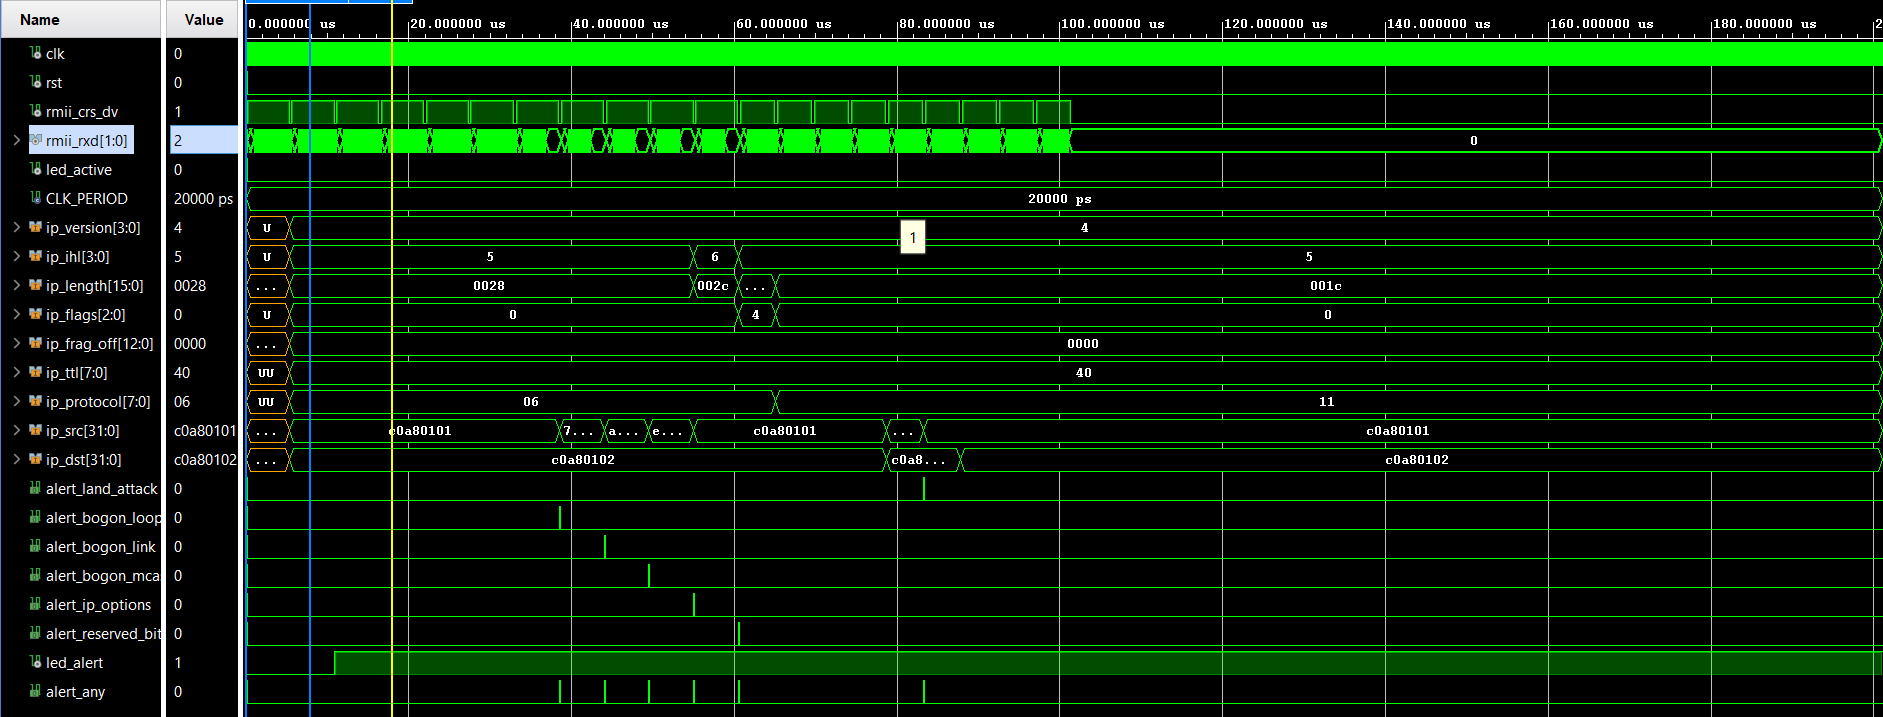
\includegraphics[width=\textwidth]{ipv4newruleswave.png}
%     \caption{Simulation waveform showing R8-R12 IPv4 IDS rules firing sequentially.}
%     \label{fig:ipv4wave}
% \end{figure}

\section{TCP Checker Verification}

Rules T1--T5 were verified by injecting five TCP frames with specific flag values and destination ports. Key test cases:

\begin{itemize}
    \item T1: \texttt{tcp\_flags = 0x03} (SYN+FIN) --- \texttt{alert\_syn\_fin} asserted.
    \item T2: \texttt{tcp\_flags = 0x06} (SYN+RST) --- \texttt{alert\_syn\_rst} asserted.
    \item T3: \texttt{tcp\_flags = 0x00} (NULL) --- \texttt{alert\_null\_scan} asserted.
    \item T4: \texttt{tcp\_flags = 0xFF} (all flags) --- \texttt{alert\_xmas\_scan} asserted.
    \item T5: \texttt{dst\_port = 23} (Telnet) --- \texttt{alert\_forbidden} asserted.
\end{itemize}

% --- FIGURE PLACEHOLDER ---
% Add your TCP checker waveform screenshot here
%
\begin{figure}[H]
     \centering
     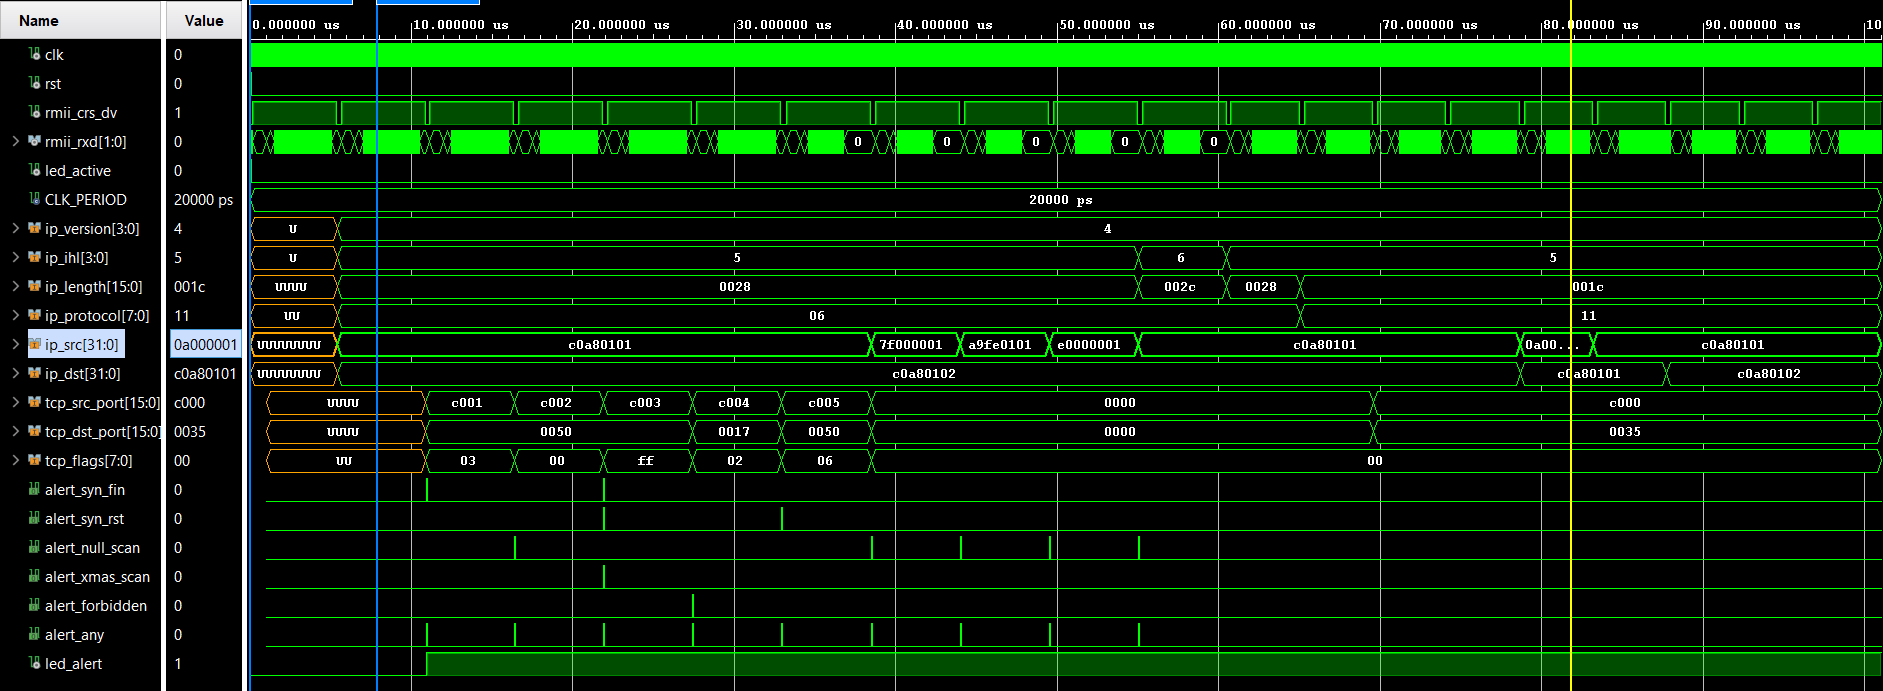
\includegraphics[width=\textwidth]{tcp_checker_waveform.png}
     \caption{Simulation waveform showing TCP rules T1--T5 firing in sequence.}
     \label{fig:tcpwave}
 \end{figure}
\section{UDP Checker}

All nine U1--U9 rules were verified by injecting dedicated UDP frames, each
violating exactly one rule while keeping all other fields valid. The rules
are grouped into three categories: forbidden port and structural checks
(U1--U3), amplification and spoofing detection (U4--U5), and size and
service abuse checks (U6--U9).

\subsection*{Forbidden Port and Structural Rules (U1--U3)}
\begin{itemize}
    \item U1: Frame with \texttt{udp\_dst\_port = 69} (TFTP, in the
          configured forbidden port table) ---
          \texttt{alert\_udp\_forbidden} asserted.
    \item U2: Frame with \texttt{udp\_length = 4} (below the minimum
          valid value of 8) --- \texttt{alert\_udp\_short} asserted.
    \item U3: Frame with \texttt{udp\_length = 0} ---
          \texttt{alert\_udp\_zero} asserted.
\end{itemize}

\subsection*{Amplification and Spoofing Rules (U4--U5)}
\begin{itemize}
    \item U4: Frame with \texttt{udp\_src\_port = 53} (DNS response
          arriving from an amplification reflector) ---
          \texttt{alert\_udp\_amplify} asserted.
    \item U5: Frame with \texttt{ip\_src = ip\_dst} and
          \texttt{udp\_src\_port = udp\_dst\_port} (UDP land attack,
          both IP-layer and port-layer conditions required simultaneously) ---
          \texttt{alert\_udp\_land} asserted. A frame satisfying only one
          of the two conditions was also sent and confirmed to produce no
          alert, verifying the AND logic of the checker.
\end{itemize}

\subsection*{Size and Service Abuse Rules (U6--U9)}
\begin{itemize}
    \item U6: Frame with \texttt{udp\_length = 1480} (exceeding the
          1472-byte MTU threshold) ---
          \texttt{alert\_udp\_oversize} asserted.
    \item U7: Frame with \texttt{udp\_dst\_port = 0} (reserved port
          zero, never valid in legitimate traffic) ---
          \texttt{alert\_udp\_port\_zero} asserted.
    \item U8: Frame with \texttt{udp\_dst\_port = 1900} (SSDP/UPnP,
          a common amplification vector) ---
          \texttt{alert\_ssdp\_abuse} asserted.
    \item U9: Frame with \texttt{udp\_dst\_port = 11211} (Memcached
          amplification request) ---
          \texttt{alert\_memcached} asserted.
\end{itemize}

In all nine cases, the alert signal was asserted within the expected
number of clock cycles from the relevant header field being assembled,
and no secondary alerts were triggered on single-violation frames.
% --- FIGURE PLACEHOLDER ---
% Add your end-to-end pipeline waveform here
%
% \begin{figure}[H]
%     \centering
%     \includegraphics[width=\textwidth]{pipeline_endtoend_waveform.png}
%     \caption{Simulation waveform showing all UDP IDS rules firing sequentially.}
%     \label{fig:e2ewave}
% \end{figure}


% ============================================================
\chapter{System Integration Architecture}
\label{ch:integration}
% ============================================================

\section{Hardware Platform}

The MicroPhase Z7-Lite board combines an ARM Cortex-A9 Processing System and Artix-7-equivalent Programmable Logic in a single Zynq-7020 SoC. The on-board Ethernet PHY (RTL8201F) connects to the PS via RGMII, meaning the MAC and PHY interface are handled entirely within the PS without consuming any PL I/O resources. This is the key constraint that shapes the integration architecture: the PL cannot directly observe the raw Ethernet wires, so raw packet bytes must be passed from PS to PL.

\begin{table}[H]
\centering
\caption{Z7-Lite pin assignments used by the PL design}
\label{tab:pins}
\begin{tabular}{lll}
\toprule
\textbf{Signal} & \textbf{Pin} & \textbf{Function} \\
\midrule
\texttt{PL\_CLK\_50M} & N18 & 50\,MHz main clock for PL logic \\
\texttt{PL\_LED1}     & P15 & \texttt{led\_alert} output       \\
\texttt{GPIO1\_17N}   & U12 & \texttt{led\_active} output      \\
\texttt{PL\_KEY1}     & P16 & Active-low reset input           \\
\bottomrule
\end{tabular}
\end{table}

\section{PS-to-PL Packet Forwarding}

The chosen integration path is:

\begin{enumerate}
    \item The PS ARM processor receives complete Ethernet frames through the GigE MAC using lwIP or a bare-metal DMA driver.
    \item The PS strips the 4-byte FCS and writes the remaining frame bytes into a DMA buffer.
    \item The AXI-Stream DMA IP transfers the buffer to PL fabric, driving an AXI-Stream slave interface.
    \item An \texttt{axis\_rx.vhd} wrapper converts the AXI-Stream handshake signals (\texttt{tvalid}, \texttt{tready}, \texttt{tdata}, \texttt{tlast}) into the four-signal byte-stream interface used internally by all IDS parsers.
\end{enumerate}

This approach keeps the entire parser and checker stack unchanged for hardware use. Only the physical reception module is swapped.

% --- FIGURE PLACEHOLDER ---
% Add your integration/co-design diagram (Image 2 from your PNGs) here
%
 \begin{figure}[H]
     \centering
     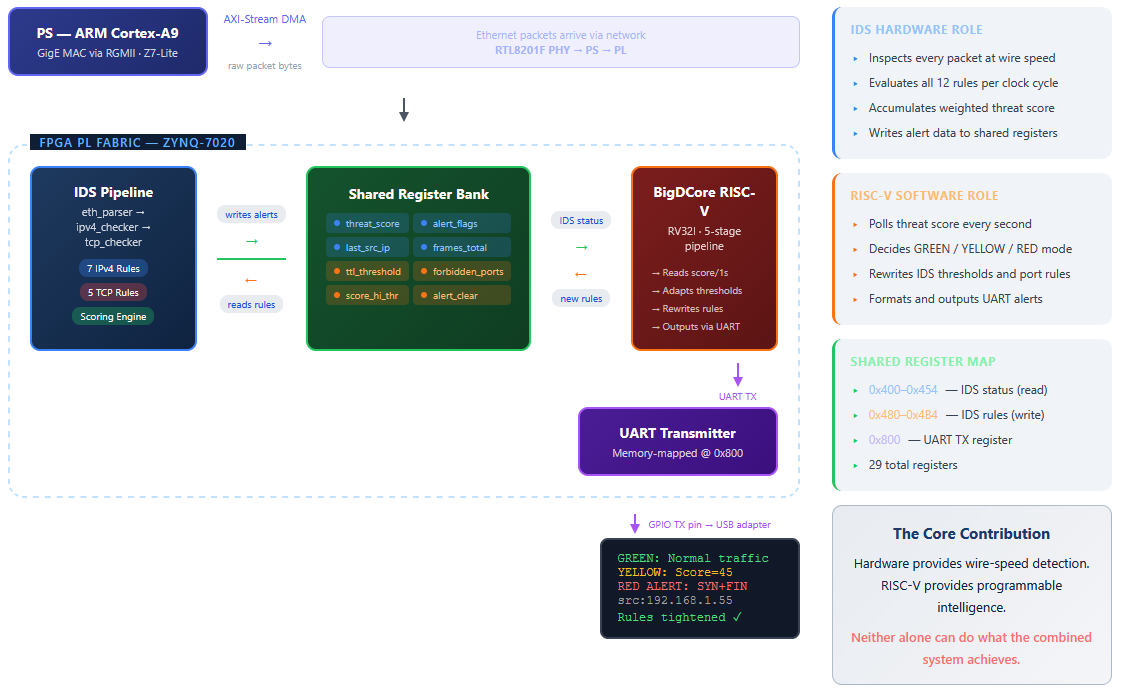
\includegraphics[width=0.95\textwidth]{integration_diagram.png}
     \caption{PS-PL co-design architecture: packet path from RTL8201F PHY through AXI-Stream DMA to the IDS pipeline, and the shared register bank connecting the IDS to the BigDCore RISC-V.}
     \label{fig:integration}
 \end{figure}

\section{AXI-Stream Wrapper (\texttt{axis\_rx.vhd})}

The AXI-Stream protocol requires a \texttt{tready} handshake from the receiver. The wrapper asserts \texttt{tready} permanently (the IDS pipeline never stalls the input stream) and maps the remaining signals directly:

\begin{itemize}
    \item \texttt{tvalid} $\rightarrow$ \texttt{rx\_valid}
    \item \texttt{tdata[7:0]} $\rightarrow$ \texttt{rx\_byte}
    \item \texttt{tlast} $\rightarrow$ \texttt{rx\_eof}
    \item A one-cycle delayed \texttt{tvalid} rising edge $\rightarrow$ \texttt{rx\_sof}
\end{itemize}

\section{RISC-V Co-Processor Integration}

\subsection{BigDCore Memory Interface}

The RISC-V processor produced by the collaborating project is named BigDCore. It implements the RV32I base integer ISA as a pipelined 32-bit processor and exposes a simple external memory interface: \texttt{DataAdr[31:0]}, \texttt{ReadData[31:0]}, \texttt{WriteData[31:0]}, \texttt{MemWrite}, \texttt{ByteEn[1:0]}, and \texttt{Mode[1:0]}. Load and store instructions drive this interface directly, so the IDS registers appear to the RISC-V as ordinary memory locations.

\subsection{Shared Register Bank}

The shared register bank (\texttt{shared\_regs.vhd}) implements 29 32-bit registers at addresses 0x400--0x4B4 in the RISC-V address space. Registers are divided into two groups:

\begin{itemize}
    \item \textbf{Status registers (0x400--0x454):} Written by the IDS hardware, read by the RISC-V. These include the threat score, a 12-bit alert flags bitmask, cumulative alert counts, per-protocol frame counts, frames-per-second statistics, and the fields of the last alerted packet (source/destination IP, ports, TCP flags, TTL, protocol, length).
    \item \textbf{Rule registers (0x480--0x4B4):} Written by the RISC-V, read by the IDS hardware. These include the TTL threshold, fragmentation check enable, scoring thresholds, score decay rate, an alert clear command, and eight configurable forbidden port values.
\end{itemize}

\begin{table}[H]
\centering
\caption{Shared register map (selected registers)}
\label{tab:regmap}
\begin{tabular}{lll}
\toprule
\textbf{Address} & \textbf{Register} & \textbf{Direction} \\
\midrule
0x400 & \texttt{threat\_score}        & IDS $\rightarrow$ RISC-V \\
0x404 & \texttt{alert\_flags}         & IDS $\rightarrow$ RISC-V \\
0x408 & \texttt{alert\_count\_total}  & IDS $\rightarrow$ RISC-V \\
0x428 & \texttt{fps\_total}           & IDS $\rightarrow$ RISC-V \\
0x434 & \texttt{last\_alert\_src\_ip} & IDS $\rightarrow$ RISC-V \\
0x454 & \texttt{threat\_level}        & IDS $\rightarrow$ RISC-V \\
0x480 & \texttt{ttl\_threshold}       & RISC-V $\rightarrow$ IDS \\
0x488 & \texttt{score\_high\_threshold} & RISC-V $\rightarrow$ IDS \\
0x490 & \texttt{score\_decay\_rate}   & RISC-V $\rightarrow$ IDS \\
0x494 & \texttt{alert\_clear}         & RISC-V $\rightarrow$ IDS \\
0x498 & \texttt{forbidden\_port\_0}   & RISC-V $\rightarrow$ IDS \\
0x800 & \texttt{uart\_tx}             & RISC-V $\rightarrow$ UART \\
\bottomrule
\end{tabular}
\end{table}

\subsection{Adaptive Threat Scoring}

The threat score accumulator adds the weight of each fired alert every clock cycle and subtracts a configurable decay rate every second. The RISC-V polls the score register at one-second intervals and maps the result to one of three severity levels:

\begin{itemize}
    \item \textbf{GREEN} (score $<$ 30): Normal traffic. Rule thresholds remain at their defaults.
    \item \textbf{YELLOW} (30 $\leq$ score $<$ 100): Elevated activity. The RISC-V tightens the TTL threshold and lowers the fragmentation detection sensitivity.
    \item \textbf{RED} (score $\geq$ 100): Active attack. The RISC-V sets the TTL threshold to its maximum and enables all optional checks.
\end{itemize}

This feedback loop means the system becomes progressively more sensitive during an attack and automatically relaxes back to baseline once the attack subsides.

\subsection{UART Alert Output}

The RISC-V formats alert data into human-readable strings and transmits them over UART through a memory-mapped transmitter at address 0x800. A typical alert message contains the severity level, the triggered rule, and the source IP address of the offending packet.

\section{Packet Capture Module (\texttt{packet\_capture.vhd})}

The packet capture module acts as a Wireshark-like header recorder. On each \texttt{frame\_done} pulse, it latches all parsed header fields (Ethernet MACs, EtherType, all IPv4 fields, ports, TCP flags, sequence number) into a set of registers accessible from the RISC-V address space. A \texttt{capture\_mode} bit selects between logging every frame and logging only frames that triggered at least one alert. The RISC-V can read these registers after each alert to reconstruct the offending packet's header for UART reporting.

\section{Future Hardware Integration Steps}

The simulation-verified pipeline is ready for hardware deployment. The remaining steps are:

\begin{enumerate}
    \item Create a Vivado block design targeting xc7z020clg400-1. Configure the Zynq PS IP for GigE MAC with DMA, add the AXI-Stream DMA IP, and connect the IDS PL design as a custom IP block.
    \item Write a minimal PS bare-metal C driver in Vitis that receives frames from the GigE MAC and forwards raw bytes to the PL via the DMA.
    \item Apply the XDC pin constraints from Table~\ref{tab:pins}.
    \item Validate with Scapy-generated test packets from a PC connected to the board over Ethernet.
\end{enumerate}

If hardware integration is not completed before the defense, the simulation demonstration is an equivalent and fully accepted validation of the IDS functionality.

% ============================================================
\chapter{Conclusion}
\label{ch:conclusion}
% ============================================================

\section{Summary of Achievements}

This project produced a fully simulation-verified hardware IDS pipeline comprising eight VHDL modules and twenty detection rules across the Ethernet, IPv4, TCP, and UDP protocol layers. Every rule was verified individually and then validated again in a full end-to-end testbench that exercises the complete chain from raw dibit input to alert latch output.

The integration architecture connects the IDS to a RISC-V co-processor through a 29-register memory-mapped bank. This gives the RISC-V read access to live traffic statistics and alert data, and write access to configurable rule parameters, without requiring any changes to the IDS hardware itself. The resulting system combines the deterministic throughput of hardware inspection with the programmable adaptability of a software processor.

\section{Academic Contribution}

Most academic hardware IDS projects present a fixed set of rules synthesized into an FPGA and verified with pre-recorded packet traces. This project goes further in two respects:

\begin{enumerate}
    \item \textbf{Runtime reconfigurability:} Detection thresholds and forbidden port lists can be updated at runtime through the RISC-V without FPGA reprogramming.
    \item \textbf{Adaptive severity:} The weighted scoring engine with decay creates a feedback loop between traffic behaviour and rule sensitivity, approximating the behaviour of an adaptive IDS in hardware.
\end{enumerate}

\section{Limitations}

The current system does not inspect packet payloads. Rules are limited to header fields, which means application-layer attacks (such as SQL injection or cross-site scripting carried in HTTP bodies) are outside the scope of detection. Additionally, the hardware integration with the Zynq PS has been designed and planned but not yet validated on physical hardware; the simulation results are the primary evidence of correctness.

\section{Future Work}

The natural extension is deep packet inspection: a \texttt{payload\_extractor.vhd} module would buffer the TCP or UDP payload into a dual-port BRAM, allowing the RISC-V to read payload bytes and search for known attack signatures. A configurable IP blacklist table stored in BRAM would allow the RISC-V to maintain a dynamic blocklist of known-malicious source addresses. ICMP parsing would add network reconnaissance detection (ping sweeps, ICMP redirect attacks). Finally, completing the hardware bring-up on the Z7-Lite would demonstrate wire-speed detection on a live network segment.

% ============================================================
%  BIBLIOGRAPHY
% ============================================================
\begin{thebibliography}{9}

\bibitem{rfc791}
J. Postel, \textit{Internet Protocol}, IETF RFC 791, September 1981.

\bibitem{rfc793}
J. Postel, \textit{Transmission Control Protocol}, IETF RFC 793, September 1981.

\bibitem{rfc768}
J. Postel, \textit{User Datagram Protocol}, IETF RFC 768, August 1980.

\bibitem{ieee8023}
IEEE Std 802.3-2022, \textit{IEEE Standard for Ethernet}, IEEE, 2022.

\bibitem{xilinxzynq}
Xilinx Inc., \textit{Zynq-7000 SoC Technical Reference Manual}, UG585, v1.13, 2022.

\bibitem{xilinxaxidma}
Xilinx Inc., \textit{AXI DMA LogiCORE IP Product Guide}, PG021, v7.1, 2021.

\bibitem{riscvspec}
A.~Waterman and K.~Asanovi\'c, \textit{The RISC-V Instruction Set Manual, Volume I: Unprivileged ISA}, RISC-V Foundation, 2019.

\bibitem{nmap}
G. Lyon, \textit{Nmap Network Scanning}, Insecure.com LLC, 2009.

\bibitem{snort}
M. Roesch, ``Snort: Lightweight intrusion detection for networks,'' in \textit{Proc. USENIX LISA}, 1999.

\end{thebibliography}

\end{document}
